%% Преамбула TeX-файла

% 1. Стиль и язык
\documentclass[utf8x, 12pt]{G7-32} % Стиль (по умолчанию будет 14pt)

% Остальные стандартные настройки убраны в preamble.inc.tex.
\sloppy

% Настройки стиля ГОСТ 7-32
% Для начала определяем, хотим мы или нет, чтобы рисунки и таблицы нумеровались в пределах раздела, или нам нужна сквозная нумерация.
\EqInChapter % формулы будут нумероваться в пределах раздела
\TableInChapter % таблицы будут нумероваться в пределах раздела
\PicInChapter % рисунки будут нумероваться в пределах раздела

% Добавляем гипертекстовое оглавление в PDF
\usepackage[
bookmarks=true, colorlinks=true, unicode=true,
urlcolor=black,linkcolor=black, anchorcolor=black,
citecolor=black, menucolor=black, filecolor=black,
]{hyperref}
\usepackage{pgfplots}
\usepackage{nomencl}

\usepackage{float}

\usepackage{indentfirst}
\setlength{\parindent}{1.25cm}

\AfterHyperrefFix

\usepackage{microtype}% полезный пакет для микротипографии, увы под xelatex мало чего умеет, но под pdflatex хорошо улучшает читаемость

% Тире могут быть невидимы в Adobe Reader
\ifInvisibleDashes
\MakeDashesBold
\fi

% Для псевдокода
\usepackage{algorithm}
\usepackage{algpseudocode}

\usepackage{graphicx}   % Пакет для включения рисунков

% С такими оно полями оно работает по-умолчанию:
% \RequirePackage[left=20mm,right=10mm,top=20mm,bottom=20mm,headsep=0pt,includefoot]{geometry}
% Если вас тошнит от поля в 10мм --- увеличивайте до 20-ти, ну и про переплёт не забывайте:
\geometry{right=10mm}
\geometry{left=30mm}
\geometry{bottom=20mm}
\geometry{ignorefoot}% считать от нижней границы текста


% Пакет Tikz
\usepackage{tikz}
\usetikzlibrary{arrows,positioning,shadows}

% Произвольная нумерация списков.
\usepackage{enumerate}

% ячейки в несколько строчек
\usepackage{multirow}

% itemize внутри tabular
\usepackage{paralist,array}

%\setlength{\parskip}{1ex plus0.5ex minus0.5ex} % разрыв между абзацами
\setlength{\parskip}{1ex} % разрыв между абзацами
\usepackage{blindtext}

% Для таблиц
\usepackage[para,online,flushleft]{threeparttable}

% Центрирование подписей к плавающим окружениям
%\usepackage[justification=centering]{caption}

\usepackage{newfloat}
\DeclareFloatingEnvironment[
placement={!ht},
name=Equation
]{eqndescNoIndent}
\edef\fixEqndesc{\noexpand\setlength{\noexpand\parindent}{\the\parindent}\noexpand\setlength{\noexpand\parskip}{\the\parskip}}
\newenvironment{eqndesc}[1][!ht]{%
    \begin{eqndescNoIndent}[#1]%
\fixEqndesc%
}
{\end{eqndescNoIndent}}

\usepackage{afterpage}

\newcommand\blankpage{
	\null
	\thispagestyle{empty}
	\newpage
}



% Настройки листингов.
\ifPDFTeX
% 8 Листинги

\usepackage{listings}

% Значения по умолчанию
\lstset{
  basicstyle= \footnotesize,
  breakatwhitespace=true,% разрыв строк только на whitespacce
  breaklines=true,       % переносить длинные строки
%   captionpos=b,          % подписи снизу -- вроде не надо
  inputencoding=koi8-r,
  numbers=left,          % нумерация слева
  numberstyle=\footnotesize,
  showspaces=false,      % показывать пробелы подчеркиваниями -- идиотизм 70-х годов
  showstringspaces=false,
  showtabs=false,        % и табы тоже
  stepnumber=1,
  tabsize=4,              % кому нужны табы по 8 символов?
  frame=single,
  xleftmargin=2.4em,
  framexleftmargin=2em
}

% Стиль для псевдокода: строчки обычно короткие, поэтому размер шрифта побольше
\lstdefinestyle{pseudocode}{
  basicstyle=\small,
  keywordstyle=\color{black}\bfseries\underbar,
  language=Pseudocode,
  numberstyle=\footnotesize,
  commentstyle=\footnotesize\it
}

% Стиль для обычного кода: маленький шрифт
\lstdefinestyle{realcode}{
  basicstyle=\scriptsize,
  numberstyle=\footnotesize
}

% Стиль для коротких кусков обычного кода: средний шрифт
\lstdefinestyle{simplecode}{
  basicstyle=\footnotesize,
  numberstyle=\footnotesize
}

% Стиль для BNF
\lstdefinestyle{grammar}{
  basicstyle=\footnotesize,
  numberstyle=\footnotesize,
  stringstyle=\bfseries\ttfamily,
  language=BNF
}

% Определим свой язык для написания псевдокодов на основе Python
\lstdefinelanguage[]{Pseudocode}[]{Python}{
  morekeywords={each,empty,wait,do},% ключевые слова добавлять сюда
  morecomment=[s]{\{}{\}},% комменты {а-ля Pascal} смотрятся нагляднее
  literate=% а сюда добавлять операторы, которые хотите отображать как мат. символы
    {->}{\ensuremath{$\rightarrow$}~}2%
    {<-}{\ensuremath{$\leftarrow$}~}2%
    {:=}{\ensuremath{$\leftarrow$}~}2%
    {<--}{\ensuremath{$\Longleftarrow$}~}2%
}[keywords,comments]

% Свой язык для задания грамматик в BNF
\lstdefinelanguage[]{BNF}[]{}{
  morekeywords={},
  morecomment=[s]{@}{@},
  morestring=[b]",%
  literate=%
    {->}{\ensuremath{$\rightarrow$}~}2%
    {*}{\ensuremath{$^*$}~}2%
    {+}{\ensuremath{$^+$}~}2%
    {|}{\ensuremath{$|$}~}2%
}[keywords,comments,strings]

% Подписи к листингам на русском языке.
\renewcommand\lstlistingname{Листинг}
\renewcommand\lstlistlistingname{Листинги}

\else
\usepackage{local-minted}
\fi

% Стиль титульного листа и заголовки
% \include{00-title}


\begin{document}

\includepdf[pages=-]{title.pdf}
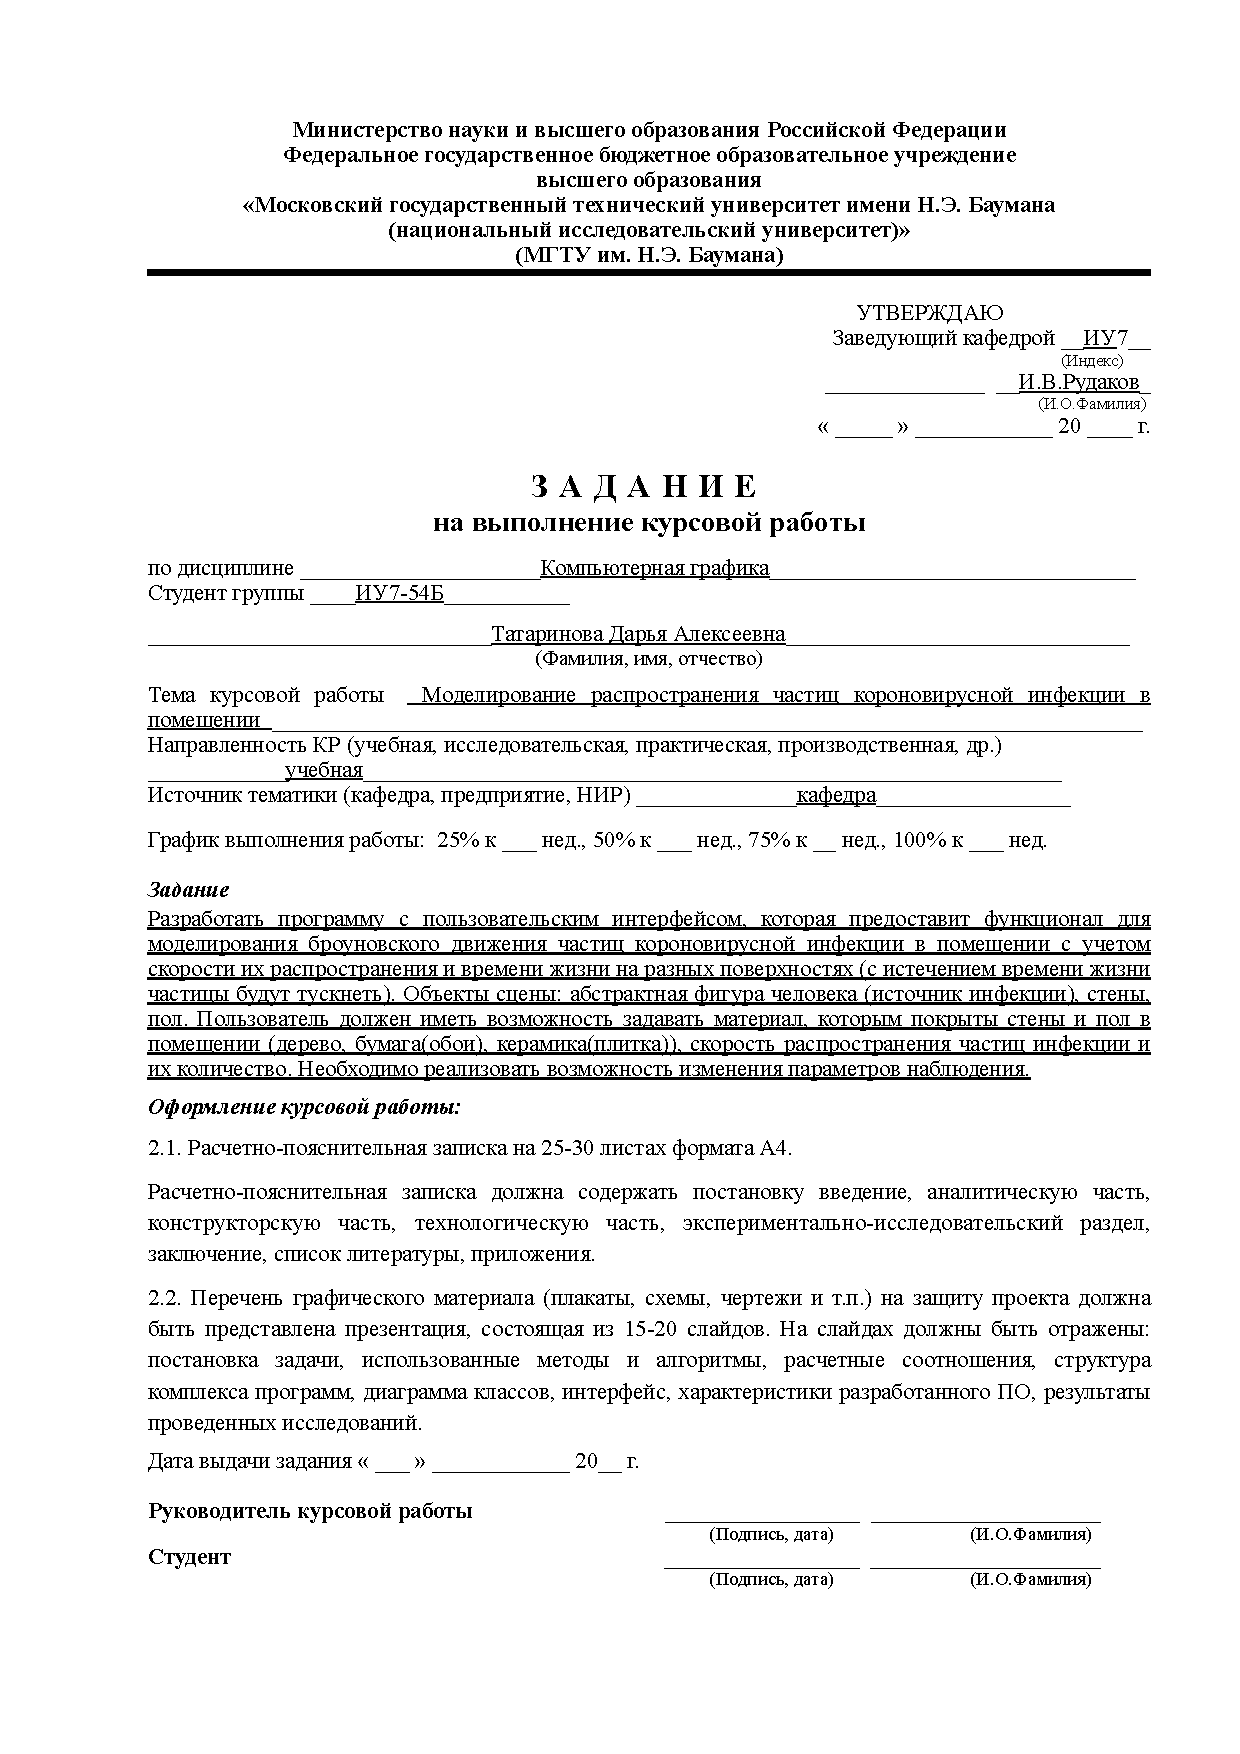
\includepdf[pages=-]{tz.pdf}

\pagenumbering{arabic}
\setcounter{page}{2}
\frontmatter % выключает нумерацию ВСЕГО; здесь начинаются ненумерованные главы: реферат, введение, глоссарий, сокращения и прочее.

%\maketitle %создает титульную страницу
% \afterpage{\blankpage}\afterpage{\blankpage}\afterpage{\blankpage}
% пропущены страницы под тз и план (у меня их 2 тз и 1 план, итого 3, вам надо пропустить столько, сколько страниц у вас в тз и плане)


%\listoffigures                         % Список рисунков

%\listoftables                          % Список таблиц

%\NormRefs % Нормативные ссылки 
% Команды \breakingbeforechapters и \nonbreakingbeforechapters
% управляют разрывом страницы перед главами.
% По-умолчанию страница разрывается.
% \Referat
%\begin{abstract}

    Отчет содержит \pageref{LastPage}\,стр.%
    \ifnum \totfig >0
    , \totfig~рис.%
    \fi
    \ifnum \tottab >0
    , \tottab~табл.%
    \fi
    %
    \ifnum \totbib >0
    , \totbib~источн.%
    \fi
    %
    \ifnum \totapp >0
    , \totapp~прил.%
    \else
    .%
    \fi


%\end{abstract}

%%% Local Variables: 
%%% mode: latex
%%% TeX-master: "rpz"
%%% End: 

% \nobreakingbeforechapters
% \breakingbeforechapters

\tableofcontents

% \printnomenclature % Автоматический список сокращений

\Introduction

С развитием компьютерных технологий компьютерная графика приобрела совершенно новый статус, поэтому сегодня она является основной технологией в цифровой фотографии, кино, видеоиграх, а также во многих специализированных приложениях. Было разработано большое количество алгоритмов отображения. Главными критериями, которые к ним предъявляются, являются реалистичность изображения и скорость отрисовки. Однако зачастую чем выше реалистичность, тем больше времени и памяти требуется для работы алгоритма.

Одним из направлений моделирования является моделирование движения частиц. Имеется огромная потребность в качественной и эффективной отрисовке распространения частиц вируса. Особенно эта тема стала актуальной после начала пандемии короновируса. Пандемия COVID-19 повлияла на жизнь миллионов людей по всему миру. Помимо серьезных последствий для здоровья, пандемия также изменила нашу повседневную жизнь, перевернула рынок вакансий и подорвала экономическую стабильность. В данном курсовом проекте речь пойдет о моделировании распространения частиц вирусной инфекции.

Цель данной курсовой работы --- разработать программу с пользовательским интерфейсом, которая предоставит функционал для моделирования броуновского движения частиц короновирусной инфекции в помещении с учетом скорости их распространения и времени жизни на разных поверхностях.

Задачи, которые необходимо выполнить для достижения поставленной цели:

\begin{itemize}
	\item изучить алгоритмы удаления невидимых линий и поверхностей и методы закраски;
	\item проанализировать алгоритмы моделирования броуновского движения;
	\item выбрать подходящие для решения поставленной задачи алгоритмы и реализовать их;
	\item формализовать модель и описать выбранные типы и структуры данных;
	\item выявить зависимость времени отрисовки кадра от количества частиц вируса, находящихся на сцене.
\end{itemize}

\mainmatter % это включает нумерацию глав и секций в документе ниже

\chapter{Аналитический раздел}
\label{cha:analysis}


В данном разделе представлено описание объектов сцены, а также обоснован выбор алгоритмов, которые будут использованы для ее визуализации.

\section{Описание и формализация объектов сцены}

\subsection{Объекты сцены}
Объекты сцены:
\begin{itemize}
	\item абстрактная фигура человека;
	\item стены;
	\item пол;
	\item частицы вируса.
\end{itemize}

Стены и пол представляют собой параллелепипеды. Частицы вируса представлены в форме шаров.

\subsection{Выбор формы представления трехмерных объектов}

Отображением формы и размеров объектов являются модели. Обычно используются три формы задания моделей:

\begin{itemize}
	\item каркасная;
	\item поверхностная;
	\item объемная.
\end{itemize}

Каркасная модель --- одна из простейших форм задания модели, так как заключается в хранении информации только о вершинах и ребрах объекта. 

Поверхностная модель объекта --- это оболочка объекта, пустая внутри. Такая информационная модель содержит данные только о внешних геометрических параметрах объекта. Такой тип модели часто используется в компьютерной графике. При этом могут использоваться различные типы поверхностей, ограничивающих объект, такие как полигональные модели, поверхности второго порядка и другие.

При объемном моделировании учитывается материал, из которого изготовлен объект. Так, известно с какой стороны поверхности расположен материал. Это реализовывается с помощью указания направления внутренней нормали.

Для решения поставленной задачи будет использована поверхностная модель, так как каркасные модели могут привести к неправильному восприятию формы объекта, а реализация объемной модели потребует большего количества ресурсов на отображение деталей, не влияющих на качество решения задачи в ее заданной формулировке.

В свою очередь поверхностная модель может задаваться параметрическим представлением или полигональной сеткой.

В случае полигональной сетки форма объекта задаётся некоторой совокупностью вершин, ребер и граней. Наиболее подходящим представлением сцены в условиях поставленной задачи будет представление в виде списка граней, так как оно позволяет проводить явный поиск вершин грани и самих граней, которые окружают вершину.

\section{Выбор и анализ алгоритмов удаления невидимых ребер и поверхностей}

\subsection{Алгоритм обратной трассировки}

Алгоритм обратной трассировки лучей отслеживает лучи в обратном направлении (от наблюдателя к объекту). Считается, что наблюдатель расположен на положительной полуоси z в бесконечности, поэтому все световые лучи параллельны оси z. В ходе работы испускаются лучи от наблюдателя и ищутся пересечения луча и всех объектов сцены. В результате, пересечение с максимальным значением z является видимой частью поверхности, и атрибуты данного объекта используются для определения характеристик пикселя, через центр которого проходит данный световой луч. 

\begin{figure}[ph!]
	\center{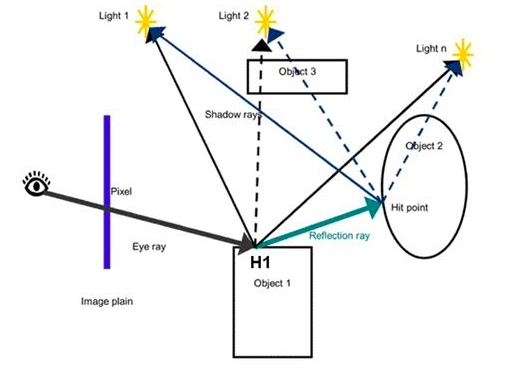
\includegraphics[scale=0.55]{img/trace.png}}
	\caption{Алгоритм обратной трассировки}
	\label{fig:trace}
\end{figure}

Эффективность процедуры определения пересечений луча с поверхностью объекта оказывает самое большое влияние на эффективность всего алгоритма. Чтобы избавиться от ненужного поиска пересечений было придумано искать пересечение луча с объемной оболочкой рассматриваемого объекта. Под оболочкой понимается некоторый простой объект, внутрь которого можно поместить рассматриваемый объект, к примеру параллелепипед или сферу. 

В дальнейшем при рассмотрении пересечения луча и объемной оболочкой рассматриваемого объекта, если такого пересечения нет, то и соответственно пересечения луча и самого рассматриваемого объекта нет, и наоборот, пересечение найдено, то возможно, есть пересечение луча и рассматриваемого объекта. 

Для расчета эффектов освещения сцены проводятся вторичные лучи от точек пересечения ко всем источникам света. Если на пути этих лучей встречается непрозрачное тело, значит данная точка находится в тени, иначе он влияет на освещение данной точки. Также для получения более реалистичного изображения сцены, нужно учитывать вклады отраженных и преломленных лучей.

Преимущества алгоритма:
\begin{itemize}
	\item возможность использования алгоритма в параллельных вычислительных системах.
\end{itemize}

Недостаттки алгоритма:
\begin{itemize}
	\item требуется большое количество высислений;
	\item производительность алгоритма.
\end{itemize}

\subsection{Алгоритм Робертса}

Алгоритм Робертса работает в объектном пространстве, кроме того работает только с выпуклыми телами. Если тело изначально является не выпуклым, то нужно его разбить на выпуклые составляющие.

Данный алгоритм состоит из следующих этапов:
\begin{itemize}
	\item подготовка исходных данных;
	\item удаление линий, экранируемых самим телом;
	\item удаление линий, экранируемых другими телами.
\end{itemize}


Для определения, лежит ли точка в положительном подпространстве, используют проверку знака скалярного произведения $(l, n)$, где $l$ --- вектор, направленный к наблюдателю, фактически определяет точку наблюдения; $n$ --- вектор внешней нормали грани. Если $(l, n) > 0$, т. е. угол между векторами острый, то грань является лицевой. Если $(l, n) < 0$, т. е. угол между векторами тупой, то грань является нелицевой.
В алгоритме Робертса требуется, чтобы все изображаемые тела или объекты были выпуклыми. Невыпуклые тела должны быть разбиты на выпуклые части. В этом алгоритме выпуклое многогранное тело с плоскими гранями должно представиться набором пересекающихся плоскостей. Уравнение произвольной плоскости в трехмерном пространстве имеет вид \ref{varnok1}.

\begin{equation}
	\label{varnok1}
	ax+by+cz+d = 0
\end{equation}

В матричной форме \ref{varnok1} выглядит как \ref{varnok2}.

\begin{equation}
	\label{varnok2}
	[x \: y \: z \: 1][P]^T = 0
\end{equation}

В формуле \ref{varnok2} выражение $[P]^T$ = $[a \; b \; c \; d]$ представляет собой плоскость. Поэтому любое выпуклое твердое тело можно выразить матрицей тела, состоящей из коэффициентов уравнений плоскостей, т. е.

\begin{equation}
	M = \begin{bmatrix}
		a_1 & a_2 & ... & a_n           \\[0.3em]
		b_1 & b_2 & ... & b_n           \\[0.3em]
		c_1 & c_2 & ... & c_n           \\[0.3em]
		d_1 & d_2 & ... & d_n           \\[0.3em]
	\end{bmatrix},
\end{equation}

где каждый столбец содержит коэффициенты одной плоскости.

Любая точка пространства может быть представлена в однородных координатах вектором $[S]~=~[x \; y \; z \; 1]$. Более того, если точка $[S]$ лежит на плоскости, то $[S]*[P]^T$ = 0. Если же $[S]$ не лежит на плоскости, то знак этого скалярного произведения показывает, по какую сторону от плоскости расположена точка. В алгоритме Робертса предполагается, что точки, лежащие внутри тела, дают отрицательное скалярное произведение, т. е. нормали направлены наружу. 

Преимущества алгоритма:
\begin{itemize}
	\item высокая точность вычислений.
\end{itemize}

Недостатки алгоритма:
\begin{itemize}
	\item рост числа трудоемкости алгоритма, как квадрата числа объектов;
	\item работа только с выпуклыми телами.
\end{itemize}

\subsection{Алгоритм, использующий Z-буфер}

Алгоритм Z-буфера решает задачу в пространстве изображений. 

В данном алгоритме рассматривается два буфера. Буфер кадра (регенерации) используется для заполнения атрибутов (интенсивности) каждого пикселя в пространстве изображения. В Z-буфер (буфер глубины) можно помещать информацию о координате z для каждого пикселя.

Для начала необходимо подготовить буферы. Для этого в Z-буфер заносятся максимально возможные значения z, а буфер кадра заполняется значениями пикселя, который описывает фон. Также нужно каждый многоугольник преобразовать в растровую форму и записать в буфер кадра. Сам процесс работы заключается в сравнении глубины каждого нового пикселя, который нужно занести в буфер кадра,
с глубиной того пикселя, который уже занесён в Z-буфер. В зависимости от сравнения принимается решение, нужно ли заносить новый пиксель в буфер кадра и, если нужно, также корректируется Z-буфер (в него нужно занести глубину нового пикселя).

Преимущества алгоритма:
\begin{itemize}
	\item элементы сцены заносятся в буфер кадра в произвольном порядке, поэтому в данном алгоритме не тратится время на выполнение сортировок;
	\item произвольная сложность сцены;
	\item поскольку размеры изображения ограничены размером экрана дисплея, трудоемкость алгоритма зависит линейно от числа рассматриваемых поверхностей.
\end{itemize}

Недостатки алгоритма:
\begin{itemize}
	\item трудоемкость устранения лестничного эффекта;
	\item трудности реализации эффектов прозрачности;
	\item большой объем требуемой памяти.
\end{itemize}


\section{Анализ методов закрашивания}

Методы закрашивания используются для затенения полигонов (или по-
верхностей, аппроксимированных полигонами) в условиях некоторой сцены, имеющей источники освещения.

Существует несколько основных методов закраски:
\begin{itemize}
	\item простая закраска;
	\item закраска по Гуро, основанная на интерполяции значений интенсивности освещенности поверхности;
	\item закраска по Фонгу, основанная на интерполяции векторов нормалей к граням многогранника.
\end{itemize}

\subsection{Простая закраска}

Одной из самых простых моделей освещения является модель Ламберта. Она учитывает только идеальное диффузное отражение света от тела. Считается, что свет падающий в точку, одинаково рассеивается по всем направлениям полупространства. Таким образом, освещенность в точке определяется только плотностью света в точке поверхности, а она линейно зависит от косинуса угла падения. При этом положение наблюдателя не имеет значение, так как диффузно отраженный свет рассеивается равномерно по всем направлениям.

Простая закраска используется при выполнении трех условий:
\begin{itemize}
	\item предполагается, что источник находится в бесконечности;
	\item предполагается, что наблюдатель находится в бесконечности;
	\item закрашиваемая грань является реально существующей, а не полученной в результате аппроксимации поверхности.
\end{itemize}

Большим недостатком данной модели является то, что все точки грани будут иметь одинаковую интенсивность.

\begin{figure}[ph!]
	\center{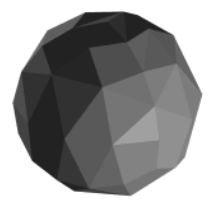
\includegraphics[scale=0.45]{img/draw_simple.png}}
	\caption{Пример простой закраскии}
	\label{fig:draw_simple}
\end{figure}

\subsection{Закраска по Гуро}

Данный алгоритм предполагает следующие шаги:

\begin{itemize}
	\item вычисление векторов нормалей к каждой грани;
	\item вычисление векторов нормали к каждой вершине грани путем усреднения нормалей к граням;
	\item вычисление интенсивности в вершинах грани;
	\item интерполяция интенсивности вдоль ребер грани;
	\item линейная интерполяция интенсивности вдоль сканирующей строки.
\end{itemize}

Достоинства:

\begin{itemize}
	\item хорошо сочетается с диффузным отражением;
	\item изображение получается более реалистичным, чем при простой закраске.
\end{itemize}

Недостатки:

\begin{itemize}
	\item данный метод интерполяции обеспечивает лишь непрерывность значений интенсивности вдоль границ многоугольников, но не обеспечивает непрерывность изменения интенсивности.
\end{itemize}

\begin{figure}[ph!]
	\center{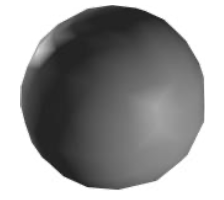
\includegraphics[scale=0.45]{img/draw_guro.png}}
	\caption{Пример закраски по Гуро}
	\label{fig:draw_guro}
\end{figure}

\subsection{Закраска по Фонгу}

При такой закраске, в отличие от метода Гуро, вдоль сканирующей строки интерполируется значение вектора нормали, а не интенсивности. 

Шаги алгоритма:

\begin{itemize}
	\item вычисление векторов нормалей в каждой грани.
	\item вычисление векторов нормали к каждой вершине грани.
	\item интерполяция векторов нормалей вдоль ребер грани.
	\item линейная интерполяция векторов нормалей вдоль сканирующей строки.
	\item вычисление интенсивности в очередной точке сканирующей строки.
\end{itemize}

Достоинства:
\begin{itemize}
	\item можно достичь лучшей локальной аппроксимации кривизны поверхности.
\end{itemize}

Недостатки:
\begin{itemize}
	\item ресурсоемкость;
	\item вычислительная сложность.
\end{itemize}


\begin{figure}[ph!]
	\center{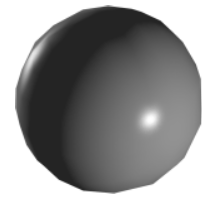
\includegraphics[scale=0.45]{img/draw_phong.png}}
	\caption{Пример закраски по Фонгу}
	\label{fig:draw_phong}
\end{figure}

\section{Алгоритмы моделирования броуновского движения}

Броуновское движение --- беспорядочное движение малых частиц, взвешенных в жидкости или газе, происходящее под действием молекул окружающей среды. 

\begin{figure}[ph!]
	\center{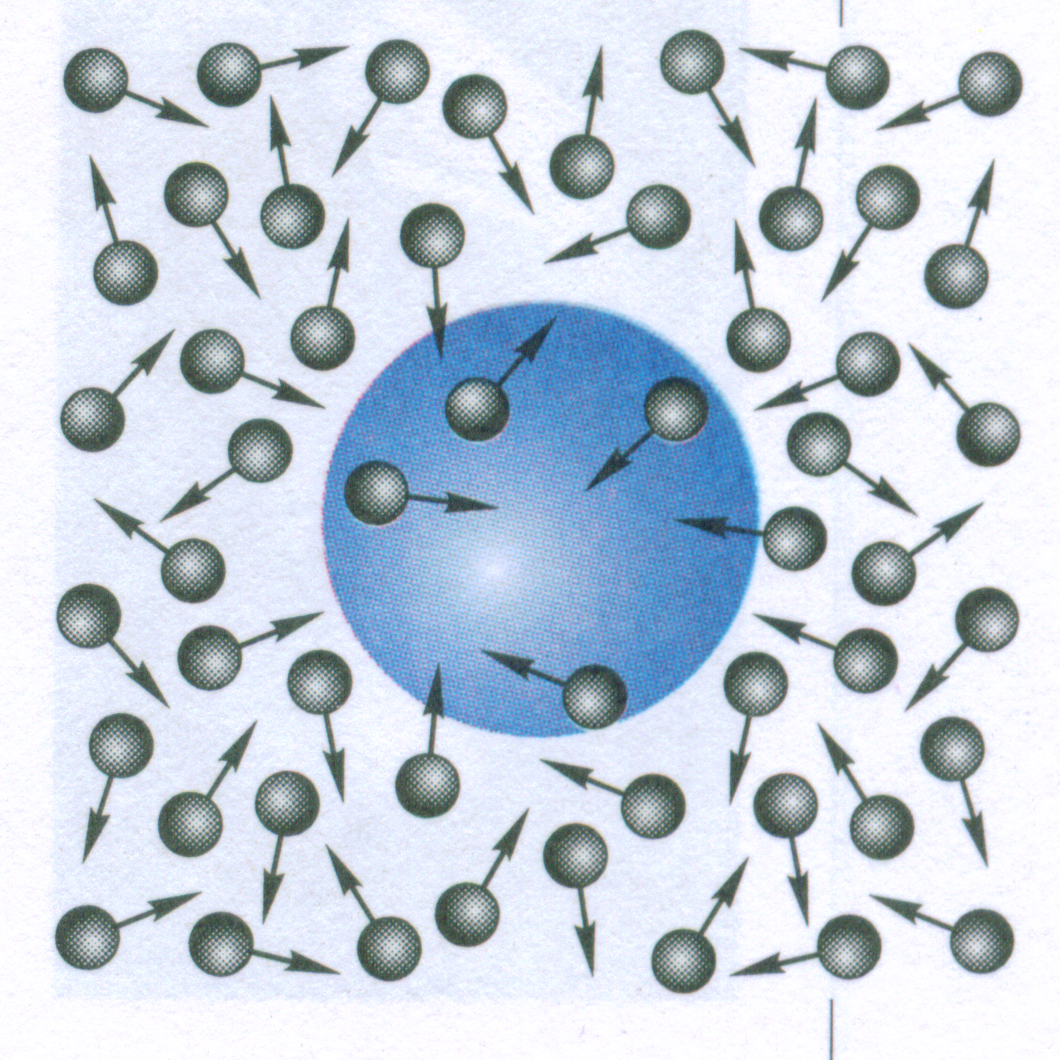
\includegraphics[scale=0.2]{img/brown_movement.png}}
	\caption{Броуновское движение}
	\label{fig:brown_movement}
\end{figure}

Рассмотрим случайный процесс (случайную величину) $X(t)$, заданную на отрезке $[0,T]$.

Случайный процесс  $X(t)$ называется одномерным броуновским движением на интервале $[0,T]$, если он обладает следущими свойствами:
\begin{itemize} 
	\item $X(0) = 0$ почти наверное и $X(t)$ - почти наверное непрерывная функция на $[0,T]$
	\item $X(t)$ - процесс с независимыми приращениями
	\item  $X(t)$ -  процесс с приращениями, распределёнными нормально.
\end{itemize}

Отметим следующие свойства броуновского движения:
\begin{itemize} 
	\item $X(t)$ почти наверное нигде не дифференцируем 
	\item  $X(t)$ - марковский процесс (не обладает памятью), т.е. если известна величина $X(t)$, то при $t_1$ < $t$ < $t_2$ величины $X(t_1)$ и $X(t_2)$ независимы.
	\item Фрактальная размерность графика $X(t)$ равна 1.5
	\item Приращение $X(t)$ обладает свойством статистического самоподобия: для любого $r > 0$
	\begin{equation}
		X(t+ \bigtriangleup t) = \frac{1}{\sqrt{r}}(X(t+r\bigtriangleup t) - X(t))
	\end{equation}
	\item Стационарность приращений: дисперсия приращения зависит только от разности моментов времени
	\begin{equation} \label{1.6}
		D(X(t_2) - X(t_1)) = \sigma^2|t_2-t_1|
	\end{equation}
	\item Математическое ожидание приращения равно
	\begin{equation}
		E(|X(t_2) - X(t_1)|) = \sqrt{\frac{2}{\pi}}\sigma\sqrt{|t_2-t_1|}
	\end{equation}
\end{itemize}

Для моделрования броуновского движения можно воспользоваться разными алгоритмами. Рассмотрим несколько из них.

\subsection{Классическое броуновское движение}

Проще всего реализовать дискретную реализацию броуновского движения, рассмотрев последовательность $x_0$ = 0, $x_{n+1} = x_n + g_n$, где $g_n$ - случайная величина, имеющая нормальное распределение (например, $N(0,1)$).

\begin{algorithmic}[1]
	\State $array[N]$
	\State $array[0]\gets 0$
	\For{i = 1,..., $N$}
	\State $array[i+1]\gets array[i] + randomNormal(0,1)$
	\EndFor
\end{algorithmic}

\subsection{Алгоритм срединных смещений}

Метод случайного срединного смещения основан на работах Н.Виннера , он более сложен, чем метод из предыдущего параграфа, однако используется для конструктивного доказательства существования броуновского движения, а также для построения фрактальной интерполяции (когда необходимо чтобы кривая проходила через заданные точки интерполяции). Метод также может быть обобщен на случай $n$-мерных броуновских движений.

Алгоритм случайного срединного смещения вычисляет значения $X(t)$ в диадических рациональных точках вида $\frac{k}{2^n}$ $\in$ [0,1]. Последовательно вычисляются значения в середине отрезка [0,1], а затем в серединах отрезков [0, $\frac{1}{2}$] и [$\frac{1}{2}, 1$] и т.д. На каждом шаге итерации должен выполнятьяс закон дисперсии для приращения в вычисленных точках. Параметр $\sigma$ определяет масщтаб по вертикальной оси, не влияя на фрактальную размерность графика. 

Вход: $N$, 	$\sigma$ // $N$ - число шагов алгоритма, при этом всего $2^N + 1$ точек интерполяции, $\sigma$ - параметр вертикального масштаба, коэффициент дисперсии

Выход: массив значений $\left\{X(\frac{k}{2^N})\right\}_{k=0}^{2^N}$ // реализация броуновского движения $X(t)$ на дискретном множестве точек вида $t_k = \frac{k}{2^N}$, k $\in$ $[0, 2^N]$

\begin{algorithmic}[1]
	\State $X(0)\gets 0$
	\State $X(1)\gets \sigma g$ // g - случайная величина, распределенная нормально с параметрами $N(0,1)$
	\For{j = 1,..., N}
	\For{i = 1,..., $2^{N-1}$}
	\State $X((2i - 1) 2^{N - j})$$\gets$ $X((i - 1)2^{N-j+1}) + X(i2^{N - j + 1}) + \frac{1}{2^{(j+1)/2}}$$\sigma$ g
	\EndFor
	\EndFor
\end{algorithmic}

\subsection{Фрактальное броуновское движение}

Фрактальное броуновское движение (ФБД) уже не является марковским процессом, а обладает некорой "памятью". Кроме того, вводя параметр $0 < H < 1$ можно получитьодномерное ФБД размерности $d = 2 - H$ и двумерное ФБД размерности $d = 3 - H$ .
Заметим, что классическое броуновское движение получается как частный случай при $H = 0.5$. Для апроксимации ФБД нет простого метода, вроде суммирования нормальных случайных величин, как в случае классического броуновского движения. Для апроксимации ФБД наиболее удобно использовать преобразования Фурье.

Рассмотрим случайный процесс (случайную величину) $X(t)$, заданную на отрезке $[0, T]$.

\textit{Случайный процесс}  $X(t)$ называется одномерным фрактальным броуновским движением на интервале $[0, T]$, если он обладает следущими свойствами:

\begin{itemize}
	\item $X(0) = 0$ почти наверное и $X(t)$ - почти наверне непрерывная функция на $[0, T]$
	\item  $X(t)$ - процесс с приращениями, распределенными нормально
\end{itemize}

Отметим следующие свойства фрактального броуновского движения:

\begin{itemize}
	\item $X(t)$ почти наверное нигде не дифференцируем 
	\item Фрактальная размерность графика $X(t)$ равна $2 - H$
	\item Процесс $x(t)$ не обладает свойством независимости приращений
	\item Приращение \textit{X(t)} обладает свойством статистического самоподобия: для любого $r$ > 0
	\begin{equation}
		X(t+ \bigtriangleup t) = \frac{1}{\sqrt{r}}(X(t+r\bigtriangleup t) - X(t))
	\end{equation}
	\item Стационарность приращений: дисперсия приращения зависит только от разности моментов времени
	\begin{equation} \label{1.6}
		D(X(t_2) - X(t_1)) = \sigma^2|t_2-t_1|^{2H}
	\end{equation}
	\item Математическое ожидание приращения равно
	\begin{equation}
		E(|X(t_2) - X(t_1)|) = \sqrt{\frac{2}{\pi}}\sigma|t_2-t_1|^H
	\end{equation}
\end{itemize}

\newtheorem{theorem1}{Теорема}
\begin{theorem1}
	Если $X(t)$ - ФБД с параметром $H$, то его спектральная плотность 
	\begin{equation}
		S(f) \propto \frac{1}{f^{2H+1}}
	\end{equation}
\end{theorem1}

Идея метода состоит в следующем. Строится преобразование Фурье для искомого ФБД в частной области, задавая случайные фазы и подбирая амплитуды, удовлетворяющие свойству из Теоремы 1. Затем получаем ФБД во временной области с помощью обратного преобразования Фурье.

Будем моделировать дискретный аналог ФБД, то есть наша цель- получить величины $\left\{X_n\right\}_{n=0}^{N-1}$, апроксимирующиеФБД в точках $n$. Воспользуемся формулой дискретного преобразования Фурье

\begin{equation}
	\hat{X_n} = \sum_{k=0}^{N-1}X_ke^{-2\pi kn/N}
\end{equation}

и обратного дискретного преобразования Фурье

\begin{equation}
	X_n = \sum_{k=0}^{N-1}\hat{X_k}e^{2\pi kn/N}
\end{equation}

Далее будем рассматривать только четные значения $N$, а для применения метода \textit{быстрого дискретного преобразования Фурье} нужно, чтобы $N=2^M$, $M \in \mathbb{N}$. Метод быстрого дискретного преобразования Фурье  реализован во многих системах компьютерной алгебры. Он позволяет сократить вычисления в $\frac{2N}{\log_2N}$ раз.

Для того, чтобы получающиеся величины $X_n$ были вещественными мы наложим условие сопряженной симметрии:

\begin{equation}
	\hat{X}_0, \hat{X}_{N/2} \in \mathbb{R}, \hat{X}_n = \hat{X}_{N-n}, n = 1,...,N/2-1
\end{equation}

Фильтрация относится к той части моделирования, когда мы заставляем коэффициенты преобразования Фурье удовлетворять степенному закону из Теоремы 1:

\begin{equation}
	|\hat{X}_n|^2 \propto \frac{1}{n^{2H+1}}, n = 1,...,N/2
\end{equation}

Для этого возьмем

\begin{equation}
	\hat{X}_n = \frac{ge^{2\pi iu}}{n^{H+0.5}}
\end{equation}

где $g$ - независимые значения нормально распределенной случайной величины с параметрами $N(0,1)$, а $u$ - независимые значения равномерно распределенной на отрезке [0,1] случайной величины. Оставшиеся коэффициенты вечислим из сотношений 1.15.

Для вычисления искомой аппроксимации ФБД $\left\{X_n\right\}_{n=0}^{N-1}$ применим обратное дискретное преобразование Фурье к набору $\left\{\hat{X}_n\right\}_{n=0}^{N-1}$.

Вход: $H \in (0,1)$, $N=2^M$, $M \in \mathbb{N}$ // $H$ - параметр ФБД, размерность графика равна $d = 2 - H$, $N$ - параметр, определяющий количество точек дискретизации ФБД.

Выход: массив значений $\left\{X_n\right\}_{n=0}^{N-1}$ // дискретная апроксимация ФБД в последовательные моменты времени n.

\begin{algorithmic}[1]
	\State $\hat{X}_0\gets g$
	\For{j = 1,..., N/2-1}
	\State $\hat{X}_j \gets \frac{ge^{2\pi iu}}{j^{H+0.5}}$
	\EndFor
	\State $\hat{X}_{N/2} \gets \frac{g\cos(2\pi iu)}{(N/2)^{H+0.5}}$ // Здесь $\cos$ — вещественная часть комплексной экспоненты $e$
	\For{j = N/2+1,..., N-1}
	\State $\hat{X}_j \gets \overline{\hat{X}_{N-j}}$
	\EndFor
	\State $X \gets convert(\hat{X})$ // Вектор $X = \left\{X_0,...,X_{N-1}\right\}$ получается обратным дискретным преобразованием Фурье из вектора $\hat{X} = \left\{\hat{X}_0,...,\hat{X}_{N-1}\right\}$.
\end{algorithmic}

\section*{Вывод}
В данном разделе было представлено описание объектов сцены, а также обоснован выбор алгоритмов, которые будут использованы для ее визуализации.

Для удаления невидимых линий и поверхностей выбран алгоритм Z-буфера, так как он обладает важными преимуществами --- высокой скоростью работы и возможностью отображать сцены произвольной сложности.
Также была выбрана локальная модель освещения Ламберта, так как программа не должна выводить реалистичного изображения и должна иметь наиболее высокую производительность, и закраска по Гуро, так как алгоритм достаточно быстр, и он хорошо сочетается с выбранным ранее Z-буфером.

Для моделирования броуновского движеняи был выбран алгоритм срединных смещений, так как он позволяет наиболее реалистично изобразить броуновское движение, а также легко обобщается для случая $n$-мерных движений. Также данный алгоритм содержит меньшее количество вычислений чем алгоритм Фурье-фильтрации, то есть вычсленяи будут выполняться быстрее. 

\chapter{Конструкторский раздел}
\label{cha:design}

В данном разделе будут представлены схемы алгоритмов, выбранных для решения задачи, и диаграмма классов.

\section{Алгоритм срединных смещений}

Схема алгоритма срединных смещений изображена на рисунке \ref{fig:brown_mov_alg}.

\begin{figure}[ph!]
	\center{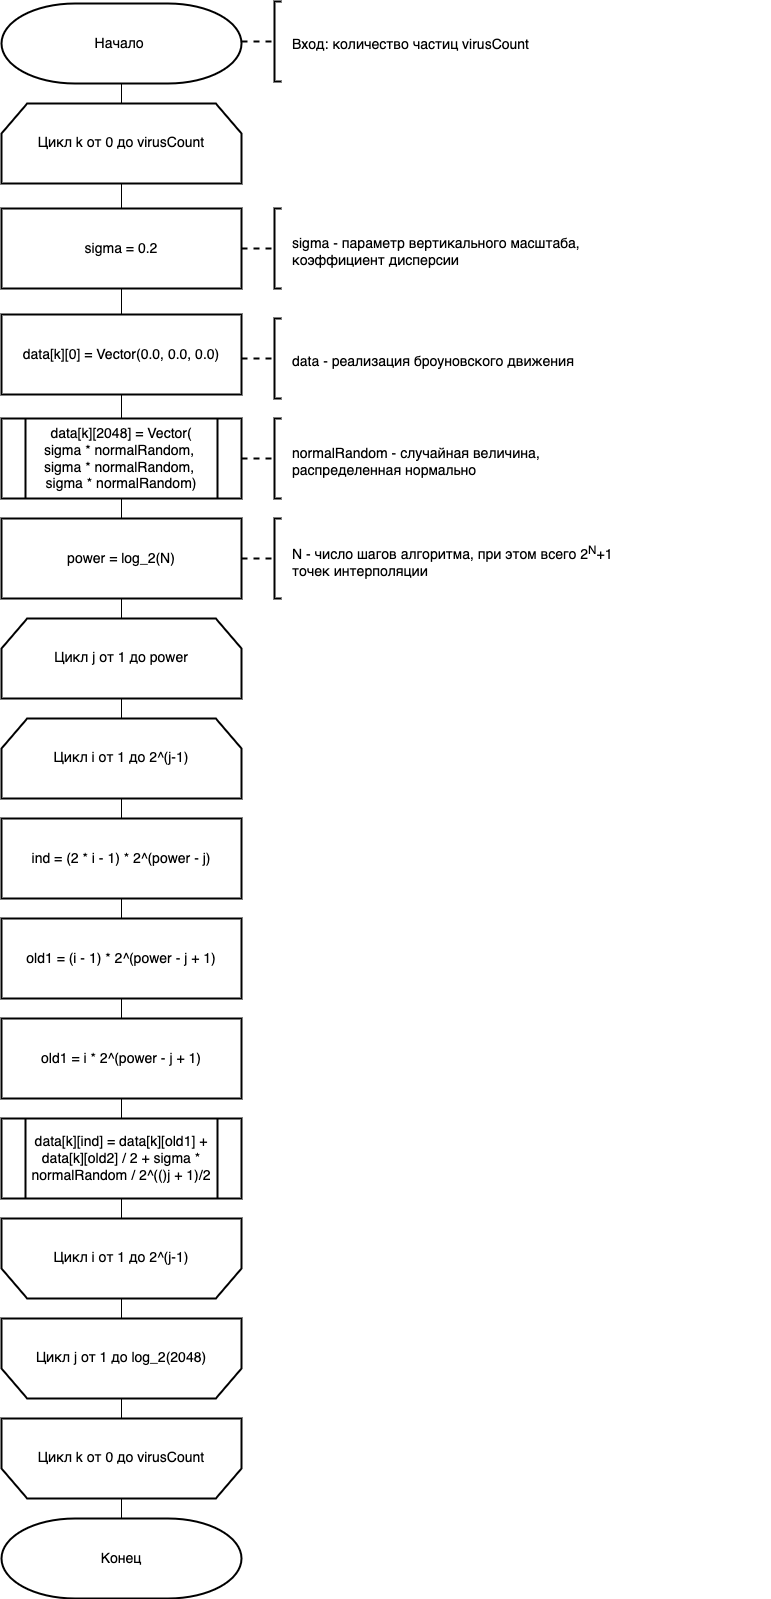
\includegraphics[scale=0.43]{img/brown.png}}
	\caption{Схема алгоритма срединных смещений}
	\label{fig:brown_mov_alg}
\end{figure}

\clearpage

\section{Алгоритмы отрисовки}

Схема алгоритма Z-буфера изображена на рисунке \ref{fig:z_buf_alg}.

\begin{figure}[ph!]
	\center{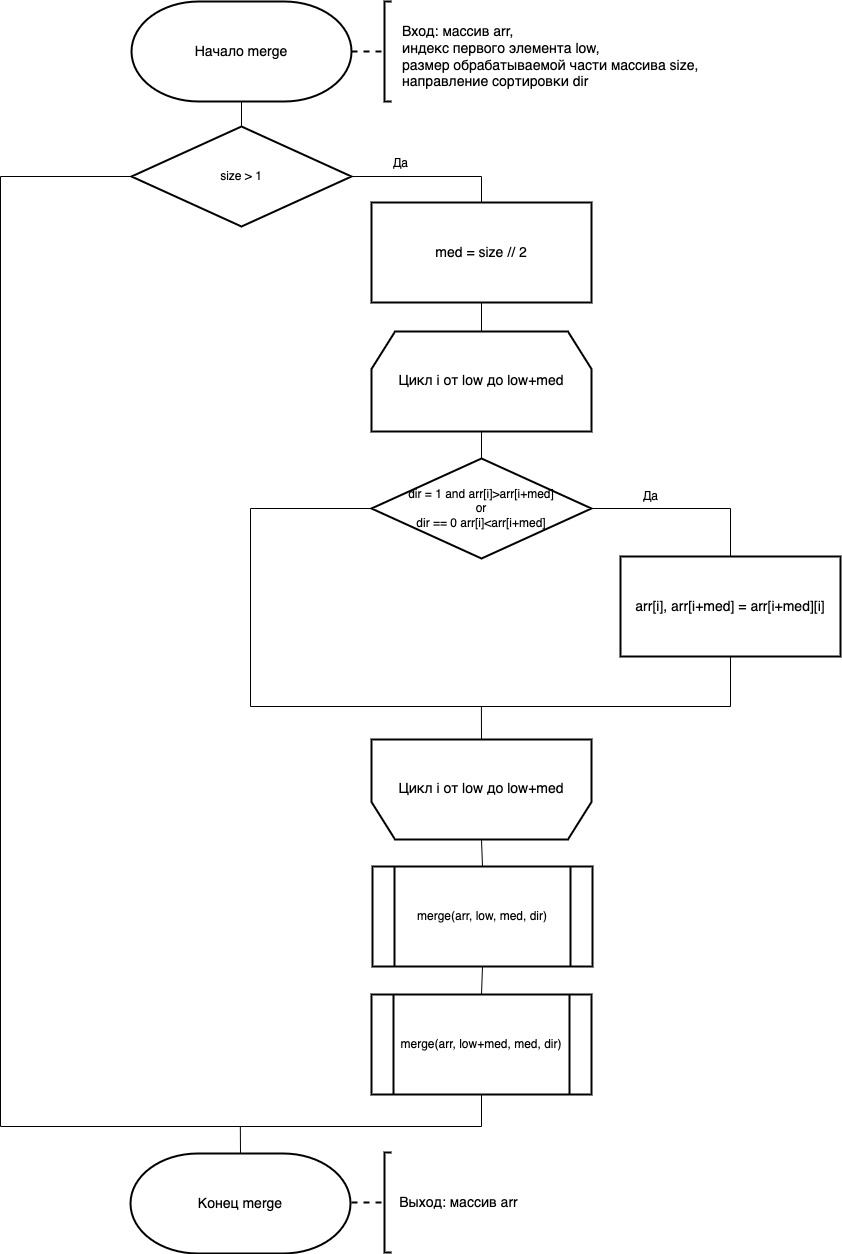
\includegraphics[scale=0.5]{img/bitonic3.png}}
	\caption{Схема алгоритма Z-буфер}
	\label{fig:z_buf_alg}
\end{figure}

\clearpage

Схема алгоритма закраски по Гуро изображена на рисунке \ref{fig:guro_alg}.

\begin{figure}[ph!]
	\center{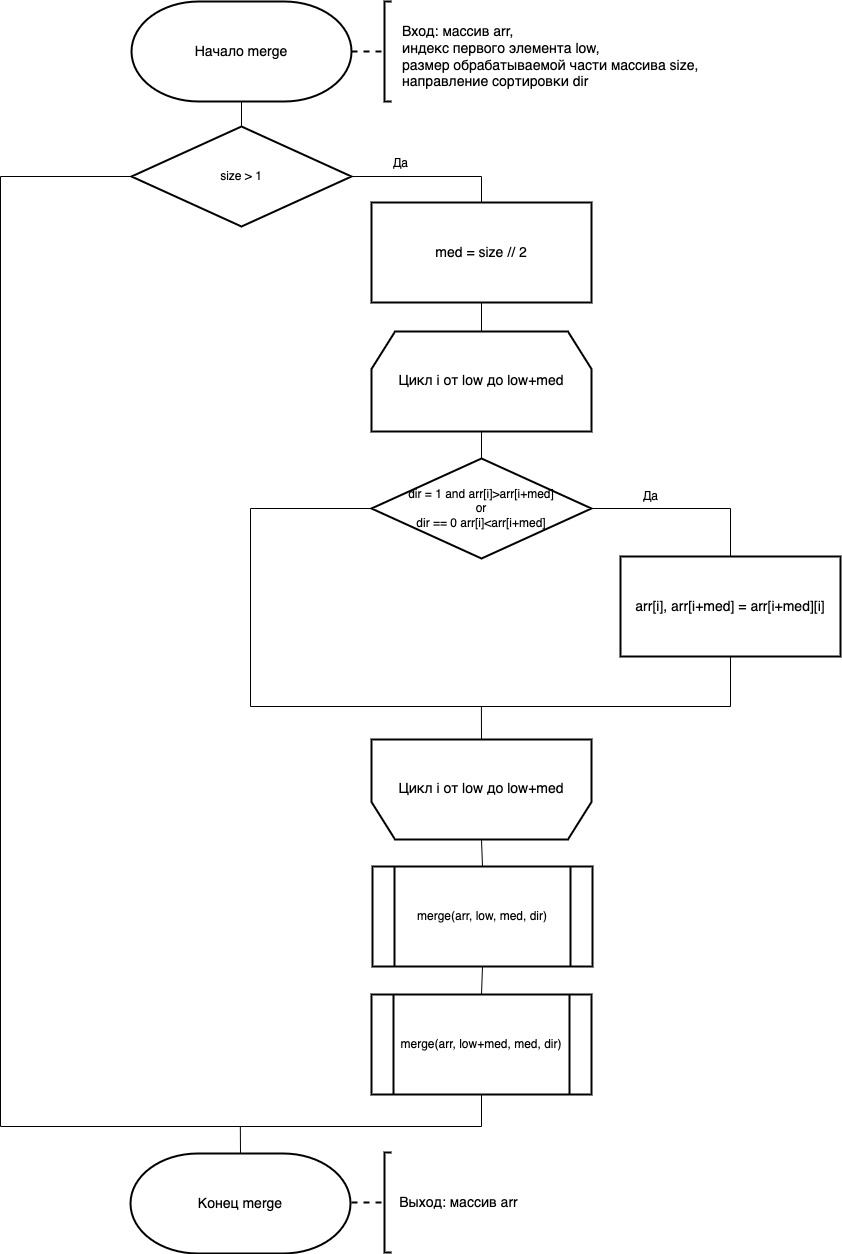
\includegraphics[scale=0.5]{img/bitonic3.png}}
	\caption{Схема алгоритма закраски по Гуро}
	\label{fig:guro_alg}
\end{figure}

\clearpage

\section{Диаграмма классов}

На рисунке \ref{fig:diag_class} представлена диаграмма классов.

\begin{figure}[ph!]
	\center{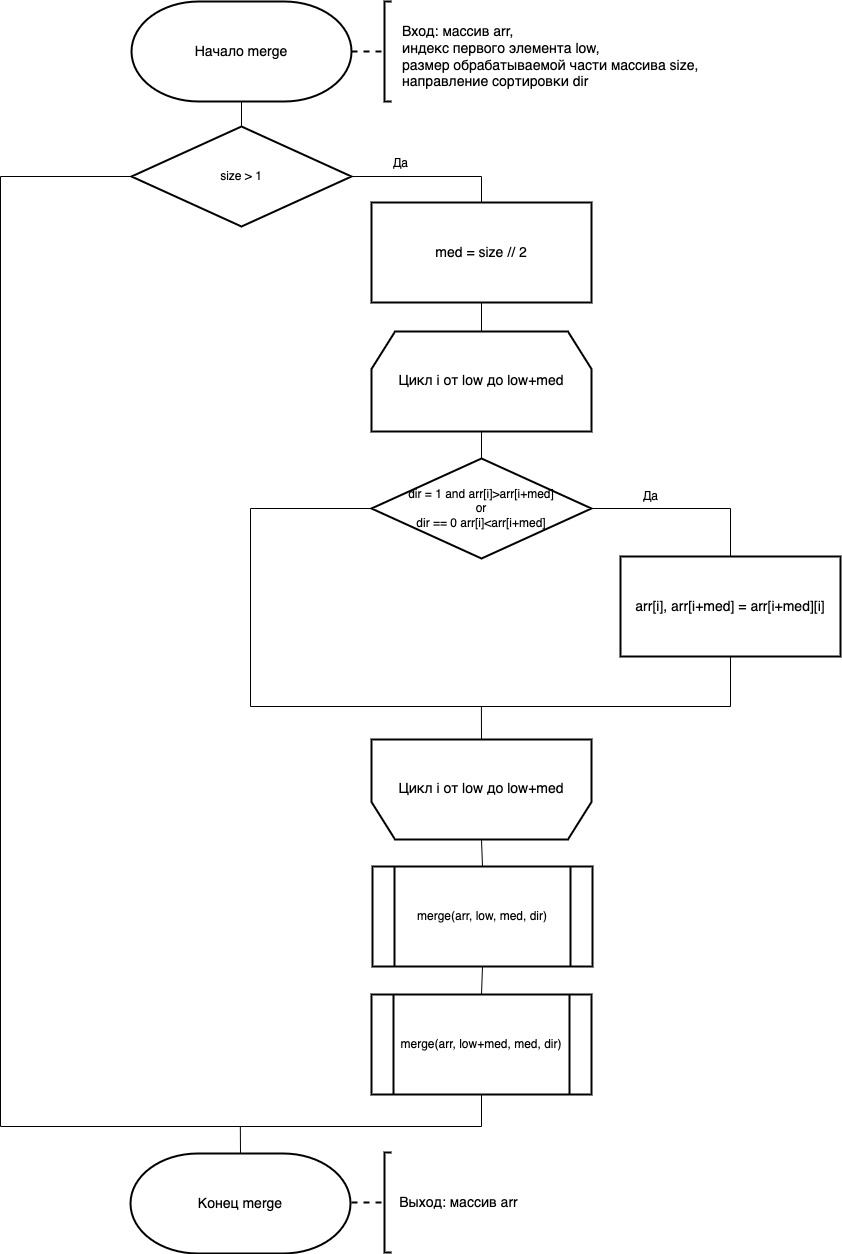
\includegraphics[scale=0.15]{img/bitonic3.png}}
	\caption{Диаграмма классов}
	\label{fig:diag_class}
\end{figure}

Классы объектов сцены:
\begin{itemize}
	\item Model (класс трёхмерных объектов с возможностью перемещения, масштабирования и поворота вокруг собственного центра);
	\item Camera (класс камеры с возможностью перемещения);
	\item LightSourcePoint (класс источника освещения с возможностью)
	перемещения по сцене и изменения мощности.
\end{itemize}

Вспомогательные классы сцены:
\begin{itemize}
	\item  Scene (контейнер, который содержит в себе объекты сцены).
\end{itemize}

\section*{Вывод}
В данном разделе были рассмотрены схемы алгоритмов, использованных при отрисовке сцены, а также диаграмма классов.



\chapter{Технологический раздел}
\label{cha:impl}

В данном разделе будет обоснован выбор языка программирования и среды разработки, представлены реализации алгоритмов и рассмотрен интерфейс программы.

\section{Требования к программному обеспечению}

Программа должна предоставлять доступ к функционалу:

\begin{itemize}
	\item возможность выбора материала покрытия пола и стен из предложенных вариантов (дерево, бумага(обои), керамика(плитка));
	\item изменение скорости движения частиц;
	\item изменение количества частиц инфекции;
	\item включение и выключение работы модели распространения частиц;
	\item вращение, перемещение и масштабирование модели.
\end{itemize}

\section{Средства реализации}

В качестве языка программирования для реализации курсовой работы использовался язык программирования C++ \cite{cplusplus}, т.к. он содержит возможности для работы с массивами и нативными потоками. В качестве среды разработки использовалась Visual Studio Code \cite{vscode}. Для замеров времени  использовалась функция time() из заголовочного файла time.h \cite{cplusplus}. Для отображения результирующих данных в виде графиков была использована библиотека языка Python matplotlib \cite{matplotlib}.

\section{Реализация алгоритмов}

В листингах \ref{code:getNormal} -- \ref{code:brown} представлена реализация алгоритмов моделирования броуновского движения и отрисовки сцены.

\begin{lstlisting}[label=code:getNormal,caption=Реализация вспомогательной функции вычисления распределенной нормально случайной величины]
float BrownianMotion::getNormalRandom()
{
	static default_random_engine e;
	static uniform_real_distribution<> dis(-0.15, 0.15);
	return dis(e);
}
\end{lstlisting}

\newpage

\begin{lstlisting}[label=code:brown,caption=Реализация расчета изменения координат центров частиц (броуновское движение)]
void BrownianMotion::setVirusCountAndResetAllIfNeeded(int newVirusCount)
{
	if (virusCount == newVirusCount)
	{
		return;
	}
	virusCount = newVirusCount;
	float sigma = 0.2;
	data = std::vector<std::vector<Vector3f>>(virusCount, std::vector<Vector3f>(SIZE + 1));
	for (int k = 0; k < virusCount; k++)
	{
		data.at(k).at(0) = Vector3f(0.0, 0.0, 0.0);
		data.at(k).at(SIZE) = Vector3f(sigma * getNormalRandom(), sigma * getNormalRandom(), sigma * getNormalRandom());
		for (int j = 1; j <= POWER; j++)
		{
			for (int i = 1; i <= pow(2, (j - 1)); i++)
			{
				int ind = (2 * i - 1) * pow(2, POWER - j);
				int old1 = (i - 1) * pow(2, POWER - j + 1);
				int old2 = i * pow(2, POWER - j + 1);
				data.at(k).at(ind).x = (data.at(k).at(old1).x + data.at(k).at(old2).x) / 2 + sigma * getNormalRandom() / pow(2, (j + 1) / 2);
				data.at(k).at(ind).y = (data.at(k).at(old1).y + data.at(k).at(old2).y) / 2 + sigma * getNormalRandom() / pow(2, (j + 1) / 2);
				data.at(k).at(ind).z = (data.at(k).at(old1).z + data.at(k).at(old2).z) / 2 + sigma * getNormalRandom() / pow(2, (j + 1) / 2);
			}
		}
	}
}
\end{lstlisting}

\section*{Вывод}
В данном разделе были перечислены требования к ПО, средства разработки, с помощью которых были реализованы последовательный и параллельный алгоритмы сортировки массивов, приведены листинги реализаций каждого из алгоритмов, а также тесты к ним.



\chapter{Исследовательский раздел}
\label{cha:research}

В данном разделе приведено сравнение алгоритмов по времени работы.
Все параметры замерялись на устройстве со следующими техническими характеристиками:
\begin{itemize}
	\item операционная система macOS Monterey 12.6 \cite{monterey};
	\item оперативная память 16 Гб;
	\item процессор 2,3 ГГц 8‑ядерный Intel Core i9 9 поколения \cite{intel}.
\end{itemize}

Во время замеров ноутбук был подключен к сети питания и нагружен только приложениями, использующимися при замерах.

\section{Измерение времени работы реализаций алгоритмов}

Процессорное время замерялось при помощи функции std::chrono::system\_clock::now() из заголовочного файла chrono~\cite{cplusplus}. Результаты сформированы в виде графиков при помощи библиотеки matplotlib~\cite{matplotlib}. 

Результаты замеров представлены в таблице \ref{tbl:timings}.

\begin{table}[h]
	\begin{center}
		\begin{threeparttable}
			\captionsetup{justification=raggedright,singlelinecheck=off}
			\caption{\label{tbl:timings} Результаты замеров}
			\begin{tabular}{|c|c|c|}
				\hline
				Количество частиц вируса& Время отрисовки сцены (в миллисекундах) \\  \hline
				1 & 235.0 \\ \hline 
				10 & 255.0 \\ \hline 
				20 & 265.0 \\ \hline 
				40 & 295.0 \\ \hline 
				60 & 330.0 \\ \hline 
				100 & 390.0 \\ \hline 
				150 & 460.0 \\ \hline 
				200 & 550.0 \\ \hline 
				250 & 620.0 \\ \hline 
				300 & 680.0 \\ \hline 
				400 & 830.0 \\ \hline 
				500 & 1000.0 \\ \hline 
				600 & 1130.0 \\ \hline 
			\end{tabular}
		\end{threeparttable}
	\end{center}
	
\end{table}

На рисунках \ref{fig:timings} на осях X указано количество частиц. Время на осях Y указано в миллисекундах.

\begin{figure}[ph!]
	\center{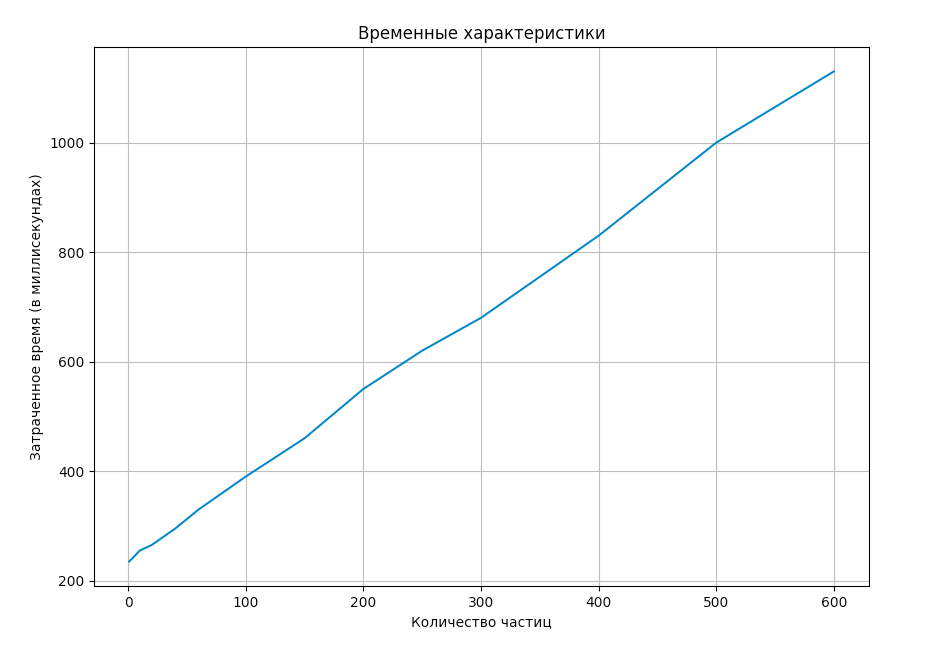
\includegraphics[scale=0.5]{img/timings.png}}
	\caption{Результаты замеров времени реализаций алгоритма битонной сортировки для разного количества потоков (количество элементов в массиве равно 1024)}
	\label{fig:timings}
\end{figure}


\section*{Вывод}

В результате эксперимента можно сделать вывод, что увеличение количества частиц вируса значительно влияет на скорость отрисовки изображения. Причем время, затрачиваемое на отрисовку сцены, линейно зависит от количества частиц.




\backmatter %% Здесь заканчивается нумерованная часть документа и начинаются ссылки и
            
\Conclusion % заключение к отчёту

В результате выполнения данной лабораторной работы была достигнута цель работы: получены навыки организации параллельных вычислений на базе нативных потоков.

Были решены все задачи:
\begin{itemize}
	\item изучены основы параллельных вычислений;
	\item реализован алгоритм битонной сортировки с использованием многопоточности и без нее;
	\item построены схемы алгоритмов;
	\item реализованы алгоритмы;
	\item проведен сравнительный анализ времени работы параллельного и последовательного алгоритмов.
\end{itemize}

В ходе сравнительного анализа самым эффективным по времени был признан параллельный алгоритм битонной сортировки. Так, при использовании 8 потоков, многопоточная реализация алгоритма битонной сортировки лучше реализации без многопоточности в среднем на 35\% при количестве элементов в массиве равном 1024.  
%% заключение


% % Список литературы при помощи BibTeX
% Юзать так:
%
% pdflatex rpz
% bibtex rpz
% pdflatex rpz

\bibliographystyle{ugost2008}
\bibliography{rpz}


%%% Local Variables: 
%%% mode: latex
%%% TeX-master: "rpz"
%%% End: 


%
\appendix   % Тут идут приложения
%
% \include{90-appendix1}
%
%\include{91-appendix2}

\end{document}

%%% Local Variables:
%%% mode: latex
%%% TeX-master: t
%%% End:
